\subsection{Naftalene}

Analoga trattazione \`e stata eseguita sul naftalene, molecola di simmetria
D$_{2h}$.
La molecola \`e stata orientata sul piano $xy$, con l'asse C$_2$ ortogonale al
piano molecolare lungo l'asse $z$.
Il calcolo \`e stato eseguito con base 6-31G* con spazio CAS 10 elettroni in
10 orbitali $\pi$ (per un totale di 4936 configurazioni) e successivamente
con base ano-1 definita 3s2p1d per il carbonio e 2s1p per l'idrogeno. Gli
orbitali facenti parte dello spazio attivo sono caratterizzati dalle
simmetrie B$_{1u}$, B$_{2g}$, B$_{3g}$, B$_{1u}$, A$_u$, B$_{2g}$, B$_{3g}$,
B$_{1u}$, A$_u$ e B$_{3g}$.  A livello HF, solo i primi 5 orbitali
(b$_{1u}$, b$_{2g}$, b$_{3g}$, b$_{1u}$, a$_u$) sono occupati.

La geometria \`e stata ottimizzata su entrambe le basi. Data l'assegnazione
per i legami data in figura

\begin{figure}[ht]
\begin{center}
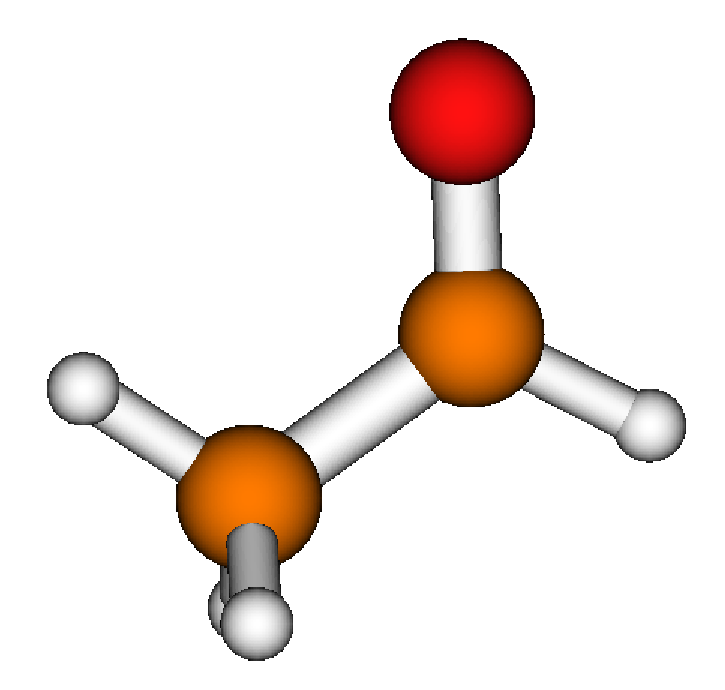
\includegraphics[angle=0,width=4cm,keepaspectratio]{immagini/naftalene/geom.eps}
\end{center}
\end{figure}

i risultati, confrontati con il valore sperimentale (Cfr. \cite{prsls-258-1960-270})
sono visibili in tabella \ref{tab:naftalene_geom}
\begin{center}
\begin{threeparttable}
\caption{\small Naftalene - geometrie su diverse basi}
\label{tab:naftalene_geom}
\small
\begin{tabular}{|l|c|c|c|}
\hline
					& 6-31G*	& ano-1		&	Exp.\tnote{1}	\\ 
\hline
$r_1$				& 1.427		& 1.427		&	1.421	\\
$r_2$				& 1.373		& 1.375		&	1.364	\\
$r_3$				& 1.421		& 1.424		&	1.415	\\
$r_4$				& 1.416		& 1.415		&	1.418	\\
\hline
\end{tabular}
\begin{tablenotes}
\small
 \item[1] Cfr. \cite{prsls-258-1960-270}
 \item[] Valori in Angstroms
\end{tablenotes}
\end{threeparttable}
\end{center}

\subsubsection{Eccitazione B$_{3u}$}

La transizione elettronica che origina lo stato eccitato di simmetria
B$_{3u}$ risulta essere quella con minima energia. Il valore sperimentale
(Cfr. \cite{cpl-16-1972-464} e \cite{jms-26-1968-67}) \`e assegnato a 4.0 eV.

La tabella \ref{tab:naftalene_b3u} mostra i risultati ottenuti con la
trattazione effettuata. Come si vede, I risultati risentono di un certo
errore rispetto al valore sperimentale.
\begin{center}
\begin{threeparttable}
\caption{\small Naftalene - Energia della transizione di simmetria B$_{3u}$. CAS
10/10 su basi differenti}
\label{tab:naftalene_b3u}
{
\begin{tabular}{|c|ccc|ccc|}
\hline
\small
 				& \multicolumn{3}{c|}{GS\tnote{1}}				& \multicolumn{3}{c|}{Ecc. B$_{3u}$\tnote{2}} \\
				& CASSCF		& NEV-PT		& NEV-PT		& CASSCF		& NEV-PT	& NEV-PT \\
				&				& SC			& PC			& 				& SC		& PC	 \\
\hline
6-31G*			& 0.477577		& 1.629822		& 1.631355		& 4.32			& 4.54		& 4.52	\\
ano-1			& 0.565924		& 1.776676		& 1.778645		& 4.29			& 4.46		& 4.43	\\
\hline
\hline
Exp.\tnote{3}	&				& 				&				& \multicolumn{3}{c|}{4.0} \\
\hline
\end{tabular}
}
\begin{tablenotes}
\small
 \item[1] Energia come \mbox{-(383 + valore)} Hartree
 \item[2] Valori in eV
 \item[3] Cfr. \cite{cpl-16-1972-464} e \cite{jms-26-1968-67}
\end{tablenotes}
\end{threeparttable}
\end{center}


\subsubsection{Eccitazione B$_{2u}$}

Per quanto riguarda l'eccitazione B$_{2u}$, i risultati sono decisamente
migliori. A livello CASSCF l'errore \`e elevato, pi\`u di 2 eV. L'applicazione
della perturbazione porta a risultati praticamente coincidenti con il range
accertato per lo sperimentale.

\begin{center}
\begin{threeparttable}
\caption{\small Naftalene - Energia della transizione di simmetria B$_{2u}$}
\label{tab:naftalene_b2u}
{
\small
\begin{tabular}{|c|ccc|}
\hline
 				& \multicolumn{3}{c|}{ Ecc. B$_{2u}$ \tnote{2}} \\
				& CASSCF		& NEV-PT & NEV-PT \\
				& 				& SC	 & PC \\
\hline
6-31G*	&  6.62			& 4.88	 &  4.82 \\
ano-1	&  6.42			& 4.51	 & 4.42	\\
\hline
\hline
Exp.\tnote{3} &	 \multicolumn{3}{c|}{4.45-4.7} \\
\hline
\end{tabular}
}
\begin{tablenotes}
\small
 \item[1] Valori in Hartree
 \item[2] Valori in eV
 \item[3] Cfr. \cite{cpl-16-1972-464}, \cite{jms-26-1968-67} e \cite{jpb-25-1992-2197}
\end{tablenotes}
\end{threeparttable}
\end{center}
